
下面的三个特性,契约、反射和模式匹配,不确定是否会成为C++23的一部分。总的想法是,它们应该是即将到来的C++标准的一部分。C++23可能会部分支持它们。

\subsubsubsection{8.2.1\hspace{0.2cm}契约}

契约本来是C++20的第五大特性。由于设计问题,在2019年7月在科隆举行的标准化委员会会议上移除。同时,创建了研究契约的\href{https://isocpp.org/std/the-committee}{第21研究组}。

\begin{itemize}
\item 
什么是契约?
\end{itemize}

契约以精确和可检查的方式,为软件组件指定接口。这些软件组件通常是函数和成员函数,必须满足前置条件、后置条件或不变式(断言)。以下是这三个术语的简化定义:

\begin{itemize}
\item 
前置条件:假定在函数输入时持有的谓词

\item 
后置条件:假定在函数退出时保持的谓词

\item 
断言:在计算中假定在其点上保持不变的谓词
\end{itemize}

前置条件和后置条件放置在函数定义之外,但不变式(断言)放置在函数定义内部。谓词是一个返回布尔值的函数。

这里是一个例子:

\begin{lstlisting}[style=styleCXX]
int push(queue& q, int val)
	[[ expects: !q.full() ]]
	[[ ensures !q.empty() ]] {
	...
	[[ assert: q.is_ok() ]]
	...
}
\end{lstlisting}

属性expect是先决条件,属性确保后置条件,属性assert是断言。函数push的契约是,在添加元素之前队列不满,在添加元素之后队列不空,并且断言q.is\_ok()成立。

前置条件和后置条件是函数接口的一部分,所以不能访问函数的局部成员或类的私有或受保护成员。然而,断言是实现的一部分,因此可以访问类的私有成员或受保护成员函数的局部变量:

\begin{lstlisting}[style=styleCXX]
class X {
public:
	void f(int n)
	[[ expects: n < m ]] // error; m is private
	{
		[[ assert: n < m ]]; // OK
		// ...
	}
private:
	int m;
};
\end{lstlisting}

成员m是私有的,因此不能成为前提条件的一部分。默认情况下,违反契约将终止程序。

并且,可以调整属性的行为。

\hspace*{\fill} \\ %插入空行
\noindent
\textbf{8.2.1.1\hspace{0.2cm}调整属性}

适配属性的语法比较复杂:[[契约属性修饰符:条件表达式]]。

\begin{itemize}
\item 
契约属性:期望、保证和断言

\item 
修饰符:指定契约级别或契约的强制执行,其值包括default、audit和axiom
\begin{itemize}
\item 
default: 运行时检查的成本应该很小,是默认的修饰符

\item 
audit: 假定运行时检查的成本很大

\item 
axiom: 运行时不检查谓词
\end{itemize}

\item 
条件表达式:契约的谓词
\end{itemize}

对于保证属性,还有一个额外的标识符可用:[[保证修饰符标识符:条件表达式]]

标识符允许引用函数的返回值。

\begin{lstlisting}[style=styleCXX]
int mul(int x, int y)
	[[expects: x > 0]] // implicit default
	[[expects default: y > 0]]
	[[ensures audit res: res > 0]] {
	return x * y;
}
\end{lstlisting}

res作为标识符是名称。如示例所示,可以使用更多相同类型的契约。

现在,来看看违反契约的处理方式。

\hspace*{\fill} \\ %插入空行
\noindent
\textbf{8.2.1.2\hspace{0.2cm}违约的处理}

编译有三个断言构建级别:

\begin{itemize}
\item 
off: 不检查契约

\item 
default: 默认检查契约

\item 
audit: 默认检查契约和审核契约
\end{itemize}

当发生违约时,由于谓词返回false,将调用违约处理程序。违约规处理程序会得到一个std::contract\_violation类型的值,此值提供关于违约的详细信息。

\begin{lstlisting}[style=styleCXX]
namespace std {
	class contract_violation{
		public:
		uint_least32_t line_number() const noexcept;
		string_view file_name() const noexcept;
		string_view function_name() const noexcept;
		string_view comment() const noexcept;
		string_view assertion_level() const noexcept;
	};
}
\end{lstlisting}

\begin{itemize}
\item 
line\_number: 违反契约的行号

\item 
file\_name: 违反契约的文件名称

\item 
function\_name: 违反契约的函数名

\item 
comment: 契约的谓词

\item 
assertion\_level: 契约的断言级别
\end{itemize}

\hspace*{\fill} \\ %插入空行
\noindent
\textbf{8.2.1.3\hspace{0.2cm}契约的声明}

契约可以放在函数的声明中,包括虚函数或函数模板的声明。

\begin{itemize}
\item 
函数的契约声明必须相同,与第一个声明不同的声明都可以省略契约。

\begin{lstlisting}[style=styleCXX]
int f(int x)
	[[expects: x > 0]]
	[[ensures r: r > 0]];

int f(int x); // OK. No contract.

int f(int x)
	[[expects: x >= 0]]; // Error missing ensures and different expects condition
\end{lstlisting}

\item 
重载函数不能修改契约。

\begin{lstlisting}[style=styleCXX]
truct B {
	virtual void f(int x)[[expects: x > 0]];
	virtual void g(int x);
};

struct D: B{
	void f(int x)[[expects: x >= 0]]; // error
	void g(int x)[[expects: x != 0]]; // error
};
\end{lstlisting}
\end{itemize}

D类契约的两个定义都是错误的。成员函数D::f的契约与B::f的契约不同,而成员函数D::g向B::g添加了一个契约。

\begin{tcolorbox}[breakable,enhanced jigsaw,colback=blue!5!white,colframe=blue!75!black,title={结束语}]
契约是C++20的一部分,但目前至少推迟到了C++23。Herb Sutter关于\href{https://herbsutter.com/2018/07/02/trip-report-summer-iso-c-standards-meeting-rapperswil/}{Sutter的话}可以让你了解了它们的重要性:“契约是迄今为止C++20中最有影响力的特性,可以说是自C++11以来,最有影响力的特性。
\end{tcolorbox}

\subsubsubsection{8.2.2\hspace{0.2cm}反射}

反射是程序分析和修改自身的可能性。反射发生在编译时,遵循C++的元规则:“不为不用的东西付费”。\href{https://en.cppreference.com/w/cpp/header/type_traits}{type-traits库}是一个用于反射的强大工具,但是用于静态反射的提案\href{http://www.open-std.org/jtc1/sc22/wg21/docs/papers/2017/p0385r2.pdf}{P0385}走得更远。

下面的代码片段应该会给你一个关于反射的直观印象:

\hspace*{\fill} \\ %插入空行
\noindent
\textbf{反射操作符}
\begin{lstlisting}[style=styleCXX]
template <typename T>
T min(constT& a,constT& b) {
	log() << "function: min<"
		  << get_base_name_v<get_aliased_t<$reflect(T)>>
		  << ">("
		  << get_base_name_v<$reflect(a)> << ": "
		  << get_base_name_v<get_aliased_t<get_type_t<$reflect(a)>>>
		  << " = " << a << ", "
		  << get_base_name_v<$reflect(b)> << ": "
		  << get_base_name_v<get_aliased_t<get_type_t<$reflect(b)>>>
		  << " = " << b
		  << ")" << '\n';
	return a < b ? a : b;
}
\end{lstlisting}

反射操作符\$reflect是示例中的关键表达式。首先,new操作符创建一个特殊的数据类型,它提供了关于模板参数T(第4行)和值a(第6行)和c(第9行)的元信息。由于函数组合,元信息可以用来提供更多信息:get\_base\_name\_v<get\_aliased\_t...(第7和第10行)。

当用参数min(12.34, 23.45)调用函数min时,会得到以下输出:

\begin{tcblisting}{commandshell={}}
function: min<double>(a: double = 12.34, b: double = 23.45)
\end{tcblisting}

读者们可能会好奇:通过反射可以获得哪些元信息?以下几点可以给你答案:

\begin{itemize}
\item 
对象:源代码行和列,以及文件名

\item 
类:私有和公共数据成员和成员函数

\item 
别名:已解析的别名
\end{itemize}

提案P0385的下一个示例展示了,反射如何帮助确定类的私有和公共成员。

\begin{lstlisting}[style=styleCXX]
#include <reflect>
#include <iostream>

struct foo {
private:
	int _i, _j;
public:
	static constexpr const bool b = true;
	float x, y, z;
private:
	static double d;
};

template <typename ... T>
void eat(T ... ) { }

template <typename Metaobjects, std::size_t I>
int do_print_data_member(void) {
	using namespace std;
	typedef reflect::get_element_t<Metaobjects, I> metaobj;
	cout << I << ": "
		<< (reflect::is_public_v<metaobj>?"public":"non-public")
		<< " "
		<< (reflect::is_static_v<metaobj>?"static":"")
		<< " "
		<< reflect::get_base_name_v<reflect::get_type_t<metaobj>>
		<< " "
		<< reflect::get_base_name_v<metaobj>
		<< '\n';
	}
	return 0;

	template <typename Metaobjects, std::size_t ... I>
	void do_print_data_members(std::index_sequence<I...>) {
		eat(do_print_data_member<Metaobjects, I>()...);
	}

	template <typename Metaobjects>
	void do_print_data_members(void) {
		using namespace std;
		
		do_print_data_members<Metaobjects>(
			make_index_sequence<
				reflect::get_size_v<Metaobjects>
			>()
		);
	}

	template <typename MetaClass>
	void print_data_members(void) {
		using namespace std;
		cout << "Public data members of " << reflect::get_base_name_v<MetaClass>
			<< '\n';
			
		do_print_data_members<reflect::get_public_data_members_t<MetaClass>>();
	}

	template <typename MetaClass>
	void print_all_data_members(void) {
		using namespace std;
		
		cout << "All data members of " << reflect::get_base_name_v<MetaClass>
			<< '\n';
		do_print_data_members<reflect::get_data_members_t<MetaClass>>();
	}

int main(void) {
	print_data_members<$reflect(foo)>();
	print_all_data_members<$reflect(foo)>();
	return 0;
}
\end{lstlisting}

该程序产生以下输出:

\begin{center}
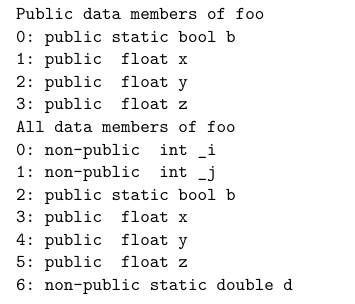
\includegraphics[width=0.5\textwidth]{content/5/chapter8/images/8.png}\\
\end{center}

\subsubsubsection{8.2.3\hspace{0.2cm}模式匹配}

诸如\href{https://en.cppreference.com/w/cpp/utility/tuple}{std::tuple}或\href{https://en.cppreference.com/w/cpp/utility/variant}{std::variant}这样的新数据类型需要新的方法来处理它们的元素。简单的if或switch条件或函数,如\href{https://en.cppreference.com/w/cpp/utility/apply}{std::apply}或\href{https://en.cppreference.com/w/cpp/utility/variant/visit}{std::visit}只能提供基本功能。函数式编程中,大量使用的模式匹配以支持更强大的新数据类型处理。

下面的代码片段来自关于模式匹配的提案\href{http://www.open-std.org/jtc1/sc22/wg21/docs/papers/2020/p1371r2.pdf}{P1371R2},比较了经典的控制结构和模式匹配。模式匹配使用关键字inspect和\_\_作为占位符。

\begin{itemize}
\item 
switch语句

\begin{lstlisting}[style=styleCXX]
switch (x) {
	case 0: std::cout << "got zero"; break;
	case 1: std::cout << "got one"; break;
	default: std::cout << "don't care";
}

inspect (x) {
	0: std::cout << "got zero";
	1: std::cout << "got one";
	__: std::cout << "don't care";
}
\end{lstlisting}

\item 
if条件语句

\begin{lstlisting}[style=styleCXX]
if (s == "foo") {
	std::cout << "got foo";
} else if (s == "bar") {
	std::cout << "got bar";
} else {
	std::cout << "don't care";
}

inspect (s) {
	"foo": std::cout << "got foo";
	"bar": std::cout << "got bar";
	__: std::cout << "don't care";
}
\end{lstlisting}

模式匹配在std::tuple、std::variant或polymorphism上的应用证明了它的强大。

\item 
std::tuple

\begin{lstlisting}[style=styleCXX]
auto&& [x, y] = p;
if (x == 0 && y == 0) {
	std::cout << "on origin";
} else if (x == 0) {
	std::cout << "on y-axis";
} else if (y == 0) {
	std::cout << "on x-axis";
} else {
	std::cout << x << ',' << y;
}

inspect (p) {
	[0, 0]: std::cout << "on origin";
	[0, y]: std::cout << "on y-axis";
	[x, 0]: std::cout << "on x-axis";
	[x, y]: std::cout << x << ',' << y;
}
\end{lstlisting}

\item 
std::variant

\begin{lstlisting}[style=styleCXX]
struct visitor {
	void operator()(int i) const {
		os << "got int: " << i;
	}
	void operator()(float f) const {
		os << "got float: " << f;
	}
	std::ostream& os;
};
std::visit(visitor{strm}, v);

inspect (v) {
	<int> i: strm << "got int: " << i;
	<float> f: strm << "got float: " << f;
}
\end{lstlisting}

\item 
多态数据类型

\begin{lstlisting}[style=styleCXX]
struct Shape { virtual ~Shape() = default; };
struct Circle : Shape { int radius; };
struct Rectangle : Shape { int width, height; };

virtual int Shape::get_area() const = 0;

int Circle::get_area() const override {
	return 3.14 * radius * radius;
}
int Rectangle::get_area() const override {
	return width * height;
}

int get_area(const Shape& shape) {
	return inspect (shape) {
		<Circle> [r] => 3.14 * r * r,
		<Rectangle> [w, h] => w * h
	}
}
\end{lstlisting}
\end{itemize}

关于模式匹配的提案P1371R2提供了更高级的用例。例如,模式匹配可用于遍历\href{https://en.wikipedia.org/wiki/Binary_expression_tree}{表达式树}。








